\documentclass[11pt]{article}

\usepackage[margin=0.88in]{geometry}
\usepackage{amsmath,amssymb}
\usepackage{booktabs}
\usepackage{graphicx}
\usepackage{xcolor}
\usepackage{microtype}
\usepackage{hyperref}
\usepackage[section]{placeins}

\hypersetup{colorlinks=true,linkcolor=blue!55!black,citecolor=blue!55!black,
  urlcolor=blue!65!black}
\setlength{\emergencystretch}{2em}
\newcommand{\Ufour}{U_4}
\newcommand{\qhat}{\widehat q}
\newcommand{\TODO}[1]{\par\medskip\noindent
  \fcolorbox{orange!70!black}{orange!7}{\parbox{0.94\linewidth}{\textbf{Open result:} #1}}
  \par\medskip}

\title{\textbf{Competing uniform and modulated order in a three-dimensional
Lifshitz scalar field theory}}
\author{Working draft---LP\_HMC collaboration}
\date{Draft of 18 November 2026}

\begin{document}
\maketitle

\begin{abstract}
We study the equilibrium phase structure of a three-dimensional real scalar
field theory containing both a conventional gradient term and a positive
biharmonic kinetic term.  A negative quadratic-gradient coefficient favors
ordering at nonzero wavevector and produces competition among a symmetric
phase, a uniform symmetry-broken phase, and a spatially modulated phase.
We use Hybrid Monte Carlo, replica exchange, umbrella reconstruction, Binder
cumulants, and shell-resolved structure factors to map this competition.
The uniform broken--symmetric line is directly resolved by finite-size Binder
crossings over a broad range of couplings.  The current direct calculation
places the termination of its conventional continuation in the narrow bare
coupling interval $-0.9625<Z_*<-0.95$.  The midpoint $Z=-0.95625$ is itself
coexistence dominated and does not support a more precise assignment.
Independent structure-factor measurements validate the detection
of finite-wavevector order, while restricted-branch thermodynamic integration
provides exploratory locations of the modulated boundaries at $L=20$.
Those restricted estimates are used only to seed unbiased finite-size scans,
not as final thermodynamic transition lines.  We set out a common
finite-size-scaling and histogram program to determine the order of all three
boundaries and to locate their junction.
\end{abstract}

\section{Introduction}

Competing interactions can move the softest fluctuations away from zero
momentum.  The resulting phase diagrams are richer than that of an ordinary
scalar $\phi^4$ theory: uniform order can compete with lamellar or more general
modulated configurations, and the associated transition lines can meet at a
Lifshitz point, a critical endpoint, a tricritical point, or a fluctuation-
induced first-order boundary.  The distinction is especially delicate in
finite periodic volumes, where only discrete momentum shells are available.

The present work asks three related questions.  First, where are the
symmetric--uniform, symmetric--modulated, and uniform--modulated transition
lines in the bare $(Z,m^2)$ plane?  Second, which transitions remain continuous
once fluctuations are included, and which become first order?  Third, how
does the familiar three-dimensional Ising critical line terminate when the
finite-wavevector mode becomes competitive?

The numerical challenge is not merely to identify a peak in a structure
factor.  Near a competing-order boundary, metastability, slow motion between
orientations, shell locking, and incomplete overlap can all imitate a sharp
transition.  We therefore combine direct finite-size observables with
distribution-level diagnostics and independent initial conditions.  Claims
about transition order are reserved for trends across several volumes.

\section{Model}

We consider a real field $\phi_x$ on a periodic cubic lattice of volume
$V=L^3$, with Hamiltonian
\begin{equation}
 H[\phi]=\sum_x\left[
 \frac{Z}{2}(\nabla\phi_x)^2+\frac12(\nabla^2\phi_x)^2
 +\frac{m^2}{2}\phi_x^2+\frac{\lambda}{4}\phi_x^4\right].
 \label{eq:H}
\end{equation}
Throughout this work $\lambda=4$ and $T=1$, and configurations have weight
$\exp[-H/T]$.  We use $m^2$ as the name of the bare mass parameter; expressions
such as $(m^2)^2$ denote its ordinary square.

For lattice momentum $k$, define
\begin{equation}
 q(k)=\widehat{k}^{,2}=4\sum_{\mu=1}^{3}\sin^2(k_\mu/2).
\end{equation}
The quadratic kernel is
\begin{equation}
 K(k)=m^2+Zq(k)+q(k)^2. \label{eq:kernel}
\end{equation}
For $Z\geq0$ its minimum is at $k=0$.  For $Z<0$, an unconstrained minimum
occurs at $q_*=-Z/2$, so that $K(k_*)=m^2-Z^2/4$.  This is a bare relation;
the observed ordering wavevector need not follow it quantitatively after
fluctuation renormalization, nonlinear mode coupling, and finite-volume
momentum quantization.

\subsection{Mean-field phase diagram}

It is useful to establish a transparent baseline.  Write $r=m^2$.  A uniform
field has free-energy density
\begin{equation}
 f_{\rm u}(v)=\frac r2v^2+\frac\lambda4v^4,
 \qquad f_{\rm u}^{\min}=-\frac{r^2}{4\lambda}\quad(r<0).
\end{equation}
For a single-mode lamellar ansatz $\phi(x)=A\cos(k_*x)$,
\begin{equation}
 f_{\rm m}(A)=\frac{r-Z^2/4}{4}A^2+\frac{3\lambda}{32}A^4,
 \qquad f_{\rm m}^{\min}=-\frac{(r-Z^2/4)^2}{6\lambda}.
\end{equation}
This approximation gives a symmetric--modulated instability at
$r=Z^2/4$ and a uniform--modulated equality line
\begin{equation}
 r=-\frac{2+\sqrt6}{4}Z^2. \label{eq:mf-um}
\end{equation}
Together with the $r=0$ symmetric--uniform line for $Z\geq0$, the three lines
meet at the mean-field Lifshitz point $(Z,r)=(0,0)$.

\begin{figure}[htbp]
 \centering
 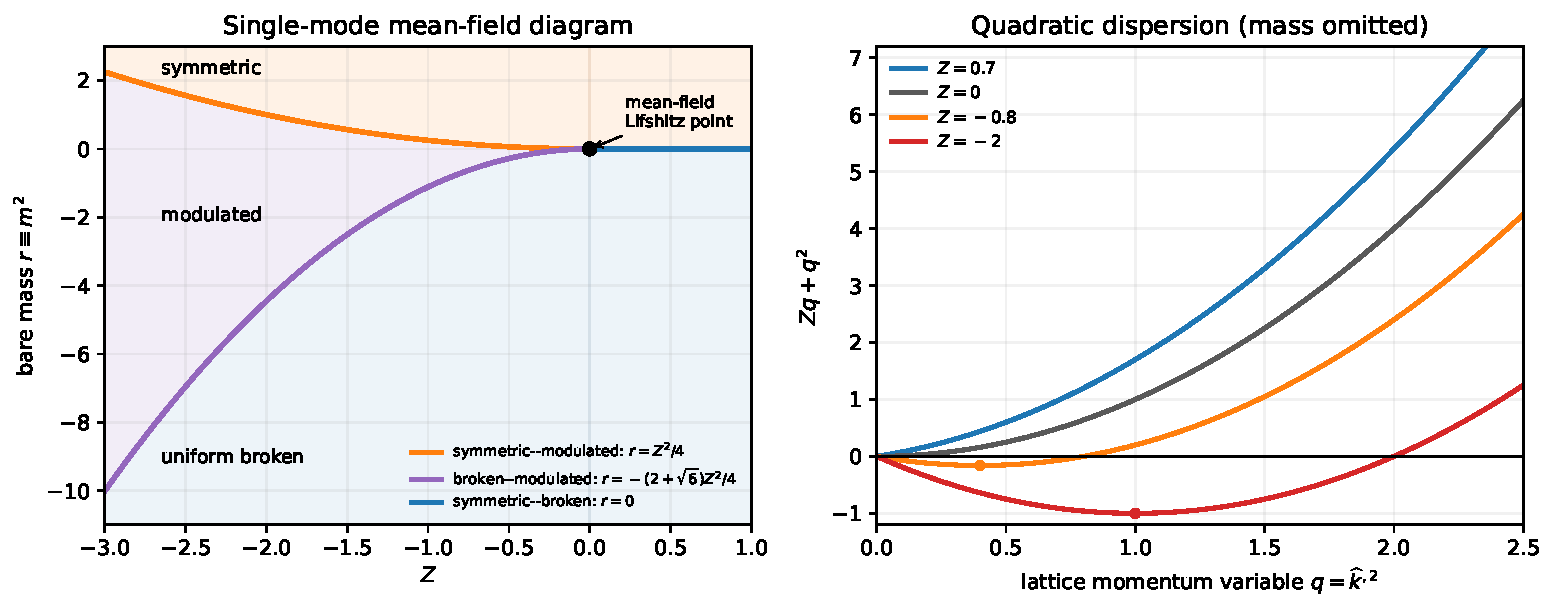
\includegraphics[width=0.98\textwidth]{generated/mean_field_phase_diagram.pdf}
 \caption{Left: single-mode mean-field phase diagram.  Right: the mass-
 independent part of the lattice quadratic kernel.  These curves are a
 baseline, not fits to the Monte Carlo phase boundaries.}
 \label{fig:mf}
\end{figure}

Several effects can change this picture.  Fluctuations shift all bare
transition lines and renormalize the preferred wavevector.  The large set of
nearly soft modes around a nonzero momentum shell can enhance fluctuations
and may drive the symmetric--modulated transition first order in the spirit
of the Brazovskii mechanism~\cite{Brazovskii1975}.  The uniform--modulated
boundary couples inequivalent order parameters and may also be discontinuous.
Conversely, the uniform symmetric transition is expected to retain
three-dimensional Ising behavior while the finite-$q$ sector remains massive.
None of these expectations substitutes for finite-size evidence in the
modified theory studied here.

\section{Numerical approach}

\subsection{Hybrid Monte Carlo}

We sample Eq.~\eqref{eq:H} with Hybrid Monte Carlo (HMC)~\cite{Duane1987}.
The molecular-dynamics force is evaluated in two lattice passes,
\begin{equation}
 F_x=Z\nabla^2\phi_x-\nabla^2(\nabla^2\phi)_x-m^2\phi_x-\lambda\phi_x^3,
\end{equation}
followed by a leapfrog trajectory and an exact Metropolis accept/reject step.
CPU and GPU implementations use the same lattice action.  Step sizes are
volume dependent and are tuned to maintain useful acceptance and
decorrelation.  Force finite differences, reversibility, energy conservation,
and acceptance sanity are tested independently before production.

\subsection{Umbrellas, replica exchange, and reweighting}

Uniform-transition calculations use overlapping umbrellas in the squared
magnetization $M^2$ and replica exchange between neighboring windows.  The
crossed-action swap probability is evaluated from
$Q=\sum_x\phi_x^2$, exactly accounting for the mass difference.  Canonical
distributions are reconstructed with the umbrella biases removed.  Each
source mass is run from at least two independent phase starts; disagreement is
treated as a convergence diagnostic rather than folded silently into a small
statistical error.

The collector retains $M^2$, $M^4$, $Q$, the energy, the gradient observable
$G=\sum_{x,\mu}(\phi_{x+\hat\mu}-\phi_x)^2$, and shell-resolved Fourier power.
This permits local reweighting in both $m^2$ and $Z$,
\begin{equation}
 w(\delta m^2,\delta Z)\propto
 \exp\left[-\frac{\delta m^2}{2T}Q-\frac{\delta Z}{2T}G\right],
\end{equation}
subject to effective-sample-size and overlap requirements.

\subsection{Restricted-branch thermodynamic integration}

To obtain efficient initial guesses in the modulated region, separate uniform
and finite-$q$ continuations are followed in mass.  Their free-energy
difference obeys
\begin{equation}
 \frac{\partial(f_a-f_b)}{\partial m^2}
 =\frac{1}{2V}\bigl(\langle Q\rangle_a-\langle Q\rangle_b\bigr).
 \label{eq:ti}
\end{equation}
Five nearby momentum shells are initialized independently, and the lowest
coherent finite-$q$ branch defines an envelope.  This construction is useful
for locating candidate scan windows.  Because it does not ensure equilibrium
transitions among all competing branches, its equality points are not by
themselves thermodynamic phase boundaries.

\section{Observables and transition diagnostics}

\subsection{Uniform order}

The uniform magnetization and Binder cumulant are
\begin{equation}
 M=\frac1V\sum_x\phi_x,\qquad
 \Ufour=1-\frac{\langle M^4\rangle}{3\langle M^2\rangle^2}.
 \label{eq:binder}
\end{equation}
Pairwise crossings between sizes locate finite-volume pseudocritical masses.
The mass derivative is obtained without numerical differencing:
\begin{equation}
 \partial_{m^2}\langle O\rangle=-\frac{1}{2T}\operatorname{Cov}(O,Q),
\end{equation}
with analytic propagation through the definition of $\Ufour$.  At a continuous
transition the slope scales approximately as
$|\partial_{m^2}\Ufour|\sim L^{1/\nu}$, up to corrections.  A first-order
transition instead produces volume scaling in appropriate response peaks and
a growing free-energy barrier.

\subsection{Finite-wavevector order}

For the Fourier transform $\widetilde\phi_k$, define total power on a lattice
shell $\mathcal S_n$ by
\begin{equation}
 P_n=\frac{1}{V^2}\sum_{k\in\mathcal S_n}|\widetilde\phi_k|^2,
 \qquad S_n=\frac{V\langle P_n\rangle}{g_n},
 \label{eq:shell}
\end{equation}
where $g_n$ is the shell degeneracy.  Summing the full shell makes $P_n$
invariant under translations, sign flips, cubic rotations, and averaging
among equivalent orientations.  The selected shell is determined from the
largest coherent $S_n$, not imposed from the bare estimate $q_*=-Z/2$.

We also monitor the shell-amplitude susceptibility, a degeneracy-normalized
Binder ratio, the fraction carried by the strongest conjugate momentum pair,
and its orientation participation ratio.  Transition classification uses
joint distributions of $(M^2,P_*)$ and of the energy.  At a candidate
first-order boundary we require stable two-phase weights and barrier growth
with interfacial area, rather than bimodality in a single histogram binning.

\begin{table}[htbp]
\centering
\caption{Common evidence required for the three boundaries.  ``Location''
means a finite-size pseudocritical estimator followed by controlled drift in
$L$; no single row alone classifies a transition.}
\label{tab:diagnostics}
\begin{tabular}{p{0.22\textwidth}p{0.27\textwidth}p{0.39\textwidth}}
\toprule
Boundary & Primary location estimator & Nature diagnostics \\
\midrule
Symmetric--uniform broken & Pairwise crossings of $\Ufour(M)$; uniform
susceptibility peak & Binder-slope exponent, susceptibility scaling,
histograms and latent-heat/barrier bounds; compare with Ising scaling \\
Symmetric--modulated & Crossings or correlation ratios built from $P_*$;
finite-$q$ susceptibility & Peak scaling, energy and $P_*$ coexistence,
barrier $\propto L^2$ versus continuous collapse; selected-$q$ drift \\
Uniform broken--modulated & Equal weight in the joint $(M^2,P_*)$
distribution & Direct switching, two-dimensional barrier, discontinuities in
$M^2$, $P_*$, $Q/V$, and energy; volume and area scaling \\
\bottomrule
\end{tabular}
\end{table}

\section{Results}

\subsection{Uniform broken--symmetric line}

Direct Binder scans for $L=12,16,20,24$ establish a smooth pseudocritical
line over $-0.5\leq Z\leq2$.  The adjacent-pair crossing masses have a spread
of roughly $0.011$--$0.017$ in $m^2$ on this grid, although the crossing
cumulants show larger corrections to scaling.  Representative curves are
shown in Fig.~\ref{fig:binder}.

\begin{figure}[htbp]
 \centering
 \begin{minipage}{0.48\textwidth}\centering
  \includegraphics[width=\linewidth]{../plots/umbrella_binder_mZm0p5_overlay.png}
  \small (a) $Z=-0.5$
 \end{minipage}\hfill
 \begin{minipage}{0.48\textwidth}\centering
  \includegraphics[width=\linewidth]{../plots/umbrella_binder_mZ1_overlay.png}
  \small (b) $Z=1$
 \end{minipage}
 \caption{Representative uniform-magnetization Binder scans.  The transition
 mass is considerably more stable than the finite-size crossing height.}
 \label{fig:binder}
\end{figure}

The direct lower-$Z$ campaign shows a robust $q=0$ crossing at $Z=-0.95$.
At $Z=-0.9625$ the formal $16\times20$ crossing is
$m^2=-2.52740$, $\Ufour=0.5122$, but it interpolates into a mass point with
large ordered/disordered source disagreement and simultaneous takeover by the
first nonzero shell.  We therefore place the current termination bracket at
\begin{equation}
 -0.9625<Z_*<-0.95. \label{eq:bracket}
\end{equation}
At the midpoint $Z=-0.95625$, a formal crossing occurs at
$m^2=-2.52025$, $\Ufour=0.6256$.  It lies only $0.0019$ above the lowest
sampled mass, which is cleanly $q=0$ dominated.  The next mass already has
severe $L=20$ source disagreement and nearly tied uniform and first-shell
power.  The interpolation therefore combines one healthy endpoint with one
contaminated endpoint and cannot defensibly tighten Eq.~\eqref{eq:bracket}.

\begin{figure}[htbp]
 \centering
 \begin{minipage}{0.48\textwidth}\centering
  \includegraphics[width=\linewidth]{../plots/binder_termination/binder_Zm0p95625_overlay.png}
  \small (a) $Z=-0.95625$
 \end{minipage}\hfill
 \begin{minipage}{0.48\textwidth}\centering
  \includegraphics[width=\linewidth]{../plots/binder_termination/binder_Zm0p9625_overlay.png}
  \small (b) $Z=-0.9625$
 \end{minipage}
 \caption{Binder reconstructions inside and at the terminated side of the
 endpoint bracket.  Formal crossings exist, but source disagreement and
 finite-$q$ takeover prevent interpreting either as a clean conventional
 critical crossing.}
 \label{fig:endpoint}
\end{figure}

The bracket is now narrower than the observed finite-size and source-history
systematics.  We therefore stop bisection and retain it as a finite-size
interval until the endpoint's volume drift and transition character are
established.

\subsection{Detection of modulated order}

The shell estimator was tested at $(Z,m^2,L)=(-4,-1,16)$, where the simulation
is trapped near a strongly modulated configuration by construction.  It
recovers the expected nonzero shell even after averaging over phase and
orientation, demonstrating that modulation is not rotated away by the
analysis.  Near the competing regime, $Z=-1$ selects a nonzero shell for
$L=16$ and $20$, while the crossing neighborhood at $Z=-0.9$ remains strongly
$q=0$ dominated.  The latter distinction is essential: a soft finite-$q$ mode
on the symmetric side does not prove that the uniform transition has already
terminated.

\begin{figure}[htbp]
 \centering
 \begin{minipage}{0.48\textwidth}\centering
  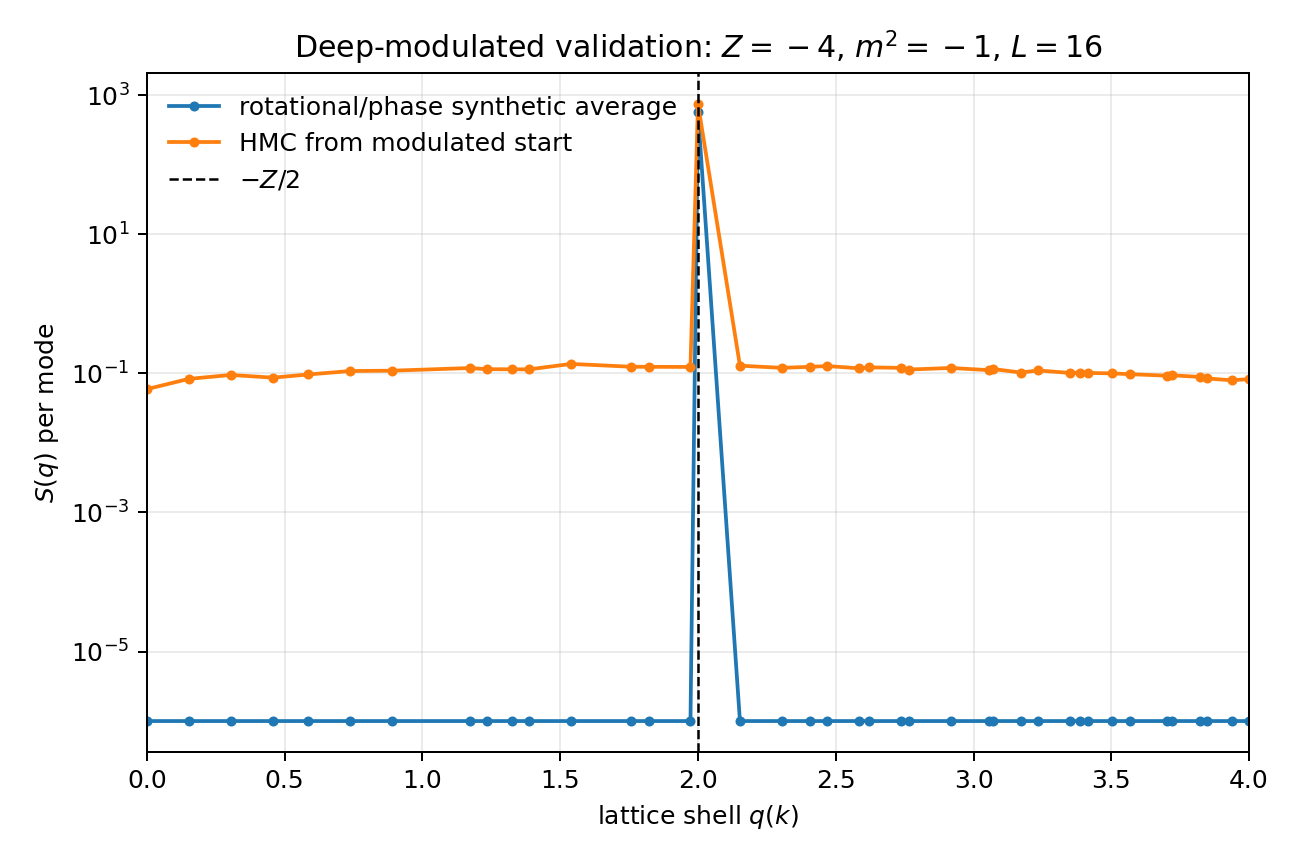
\includegraphics[width=\linewidth]{../reports/structure_factor_cpu/deep_modulated_validation/spectrum_validation.png}
  \small (a) deep-modulated validation
 \end{minipage}\hfill
 \begin{minipage}{0.48\textwidth}\centering
  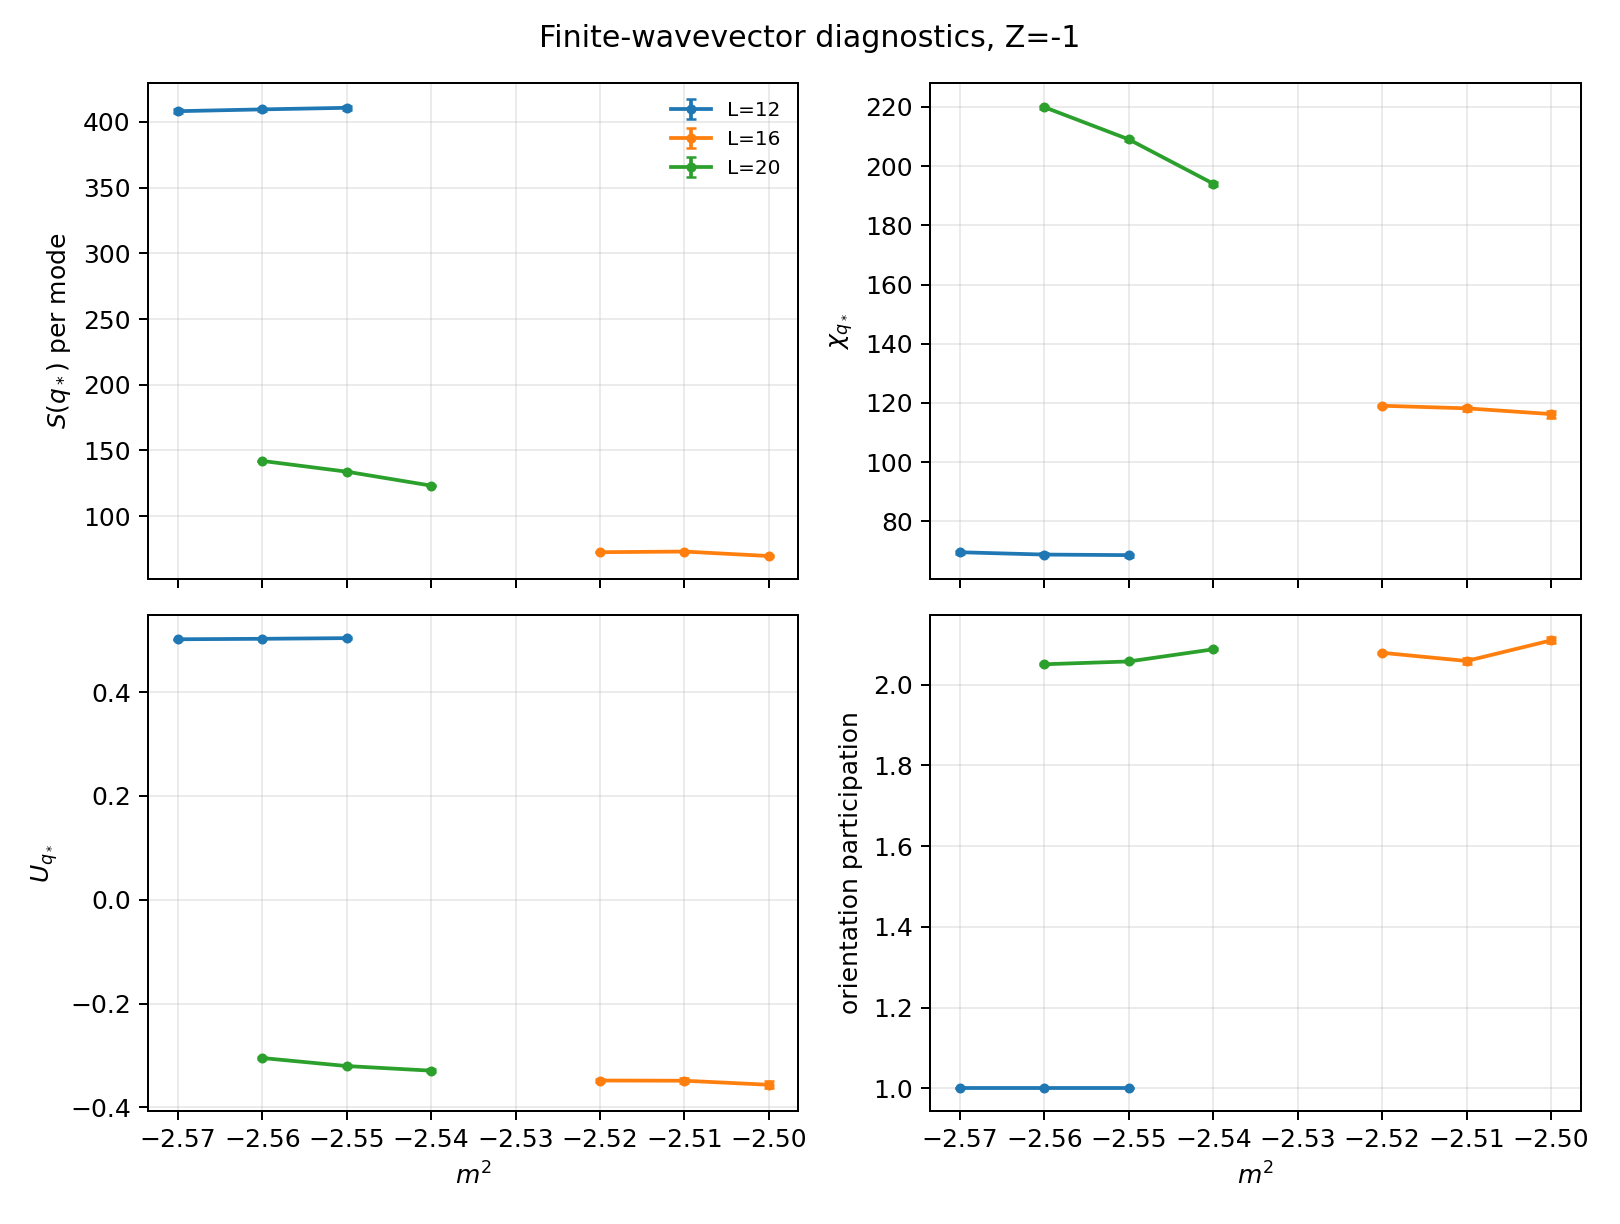
\includegraphics[width=\linewidth]{../reports/structure_factor_cpu/analysis/figures/finite_q_Zm1p0.png}
  \small (b) finite-$q$ response near $Z=-1$
 \end{minipage}
 \caption{The shell-summed structure factor detects nonzero-wavevector order
without choosing an orientation in advance.}
 \label{fig:sf}
\end{figure}

\subsection{Current phase-diagram status}

Figure~\ref{fig:status} combines three deliberately distinct evidence levels.
The blue points are direct uniform Binder crossings.  The purple line is an
$L=20$ equal-free-energy estimate between separately continued uniform and
finite-$q$ branches.  The orange line is only the point at which the chosen
finite-$q$ coherence proxy falls below threshold.  The latter two locate
promising windows but are not yet unbiased transition measurements.

\begin{figure}[htbp]
 \centering
 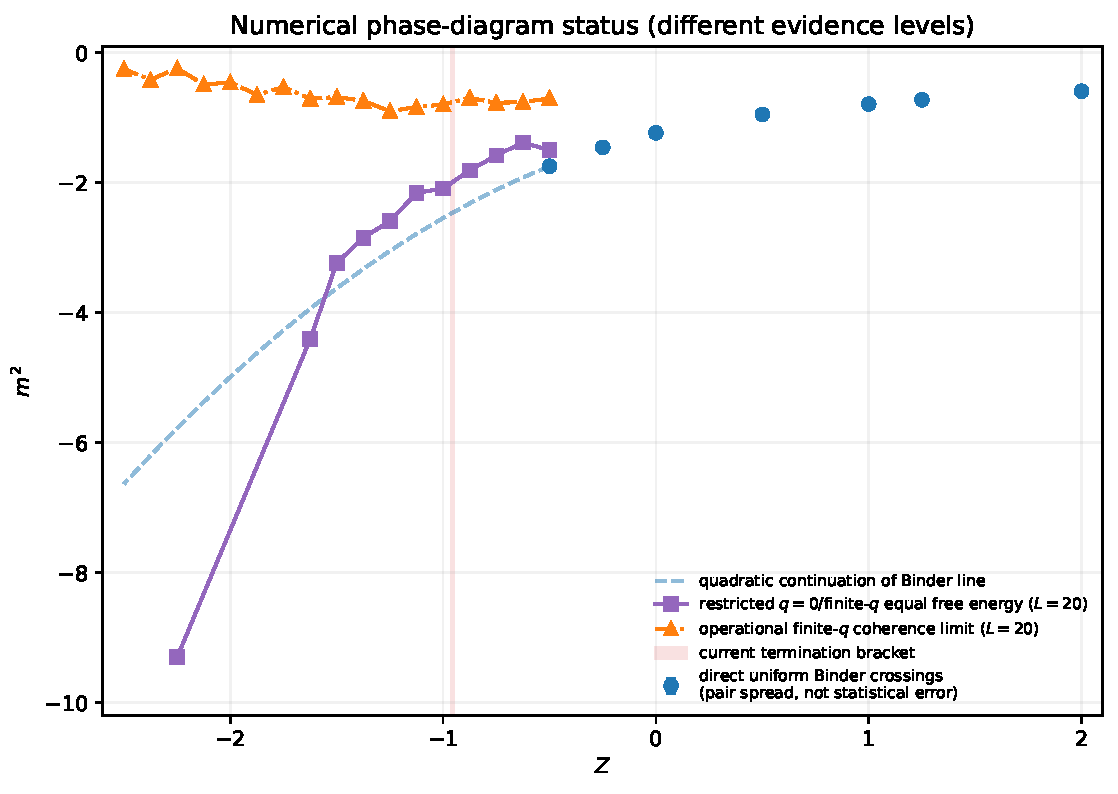
\includegraphics[width=0.82\textwidth]{generated/phase_diagram_status.pdf}
 \caption{Numerical phase-diagram status.  Direct finite-size measurements,
restricted-branch estimates, and operational proxies are shown with different
symbols because their inferential status is different.}
 \label{fig:status}
\end{figure}

The restricted multi-shell calculation finds an apparent uniform--modulated
equality curve from $Z=-0.5$ through $Z=-1.625$, with substantial lattice-shell
and continuation-history effects outside the most stable interval.  Its
intersection with the older extrapolated Binder line near $Z\simeq-1.57$ is
superseded for endpoint location by the direct bracket in
Eq.~\eqref{eq:bracket}; it remains useful as evidence that extrapolating the
uniform line deep into negative $Z$ is unsafe.  A machine-readable catalog of
all plotted points, including their evidence class and source, accompanies
this draft.

\subsection{Nature of the three transitions}

For the symmetric--uniform boundary, the working hypothesis is a continuous
three-dimensional Ising transition wherever finite-$q$ fluctuations remain
noncritical.  Existing Binder curves and derivative machinery support this
hypothesis but a final exponent analysis with stable correlated bootstrap
errors is still required.

\TODO{Symmetric--uniform: insert joint fits of Binder slopes and susceptibility
peaks for at least three sizes, correction-to-scaling sensitivity, and a table
of effective $1/\nu$.}

The symmetric--modulated transition is expected to be particularly sensitive
to the shell of soft modes.  Its classification will use finite-$q$ response
peaks and equal-weight histograms across $L=12,16,20,24$.  A first-order claim
will require response scaling compatible with $V$, stable coexistence in both
$P_*$ and energy, and a barrier increasing with $L^2$.

\TODO{Symmetric--modulated: insert direct shell-amplitude scans, pseudocritical
masses, selected wavevectors, peak/barrier scaling, and a continuous-versus-
first-order model comparison.}

The uniform--modulated boundary is a competition between nonzero $M$ and
nonzero $P_*$.  One-dimensional cuts can miss the relevant path; the decisive
object is the joint free-energy surface
$-\log P(M^2,P_*)$.  Restricted thermodynamic integration supplies initial
mass windows, after which simulations must demonstrate actual switching or a
reconstruction with connected overlap.

\TODO{Uniform--modulated: insert joint $(M^2,P_*)$ distributions, equal-weight
locations, discontinuities, interfacial barrier scaling, and finite-size drift
of the boundary.}

\section{Planned finite-size phase-map campaign}

The first production domain is $-2.5\leq Z\leq-0.5$.  The anchor values are
\begin{equation*}
 Z=-0.5,-0.75,-1.0,-1.25,-1.5,-1.75,-2.0,-2.25,-2.5,
\end{equation*}
augmented by the endpoint grid near Eq.~\eqref{eq:bracket}.  At each $Z$, restricted-branch
results define two mass windows: one around uniform--modulated competition and
one around loss of modulated order.  Discovery uses $L=12,16,20$; $L=24$ is
reserved for representative points and all putative changes of order.

Every point records $(M^2,P_*,H,Q,G)$ and orientation diagnostics.  The scan is
adaptive in $m^2$: a coarse pass brackets response peaks or equal-weight
points, then correlated reweighting is used only inside verified overlap.
Independent uniform, modulated, and symmetric starts are compared.  A point
is promoted to finite-size scaling only after source agreement or an explicit
equilibrium coexistence reconstruction.

The campaign is ordered to answer the physics efficiently:
\begin{enumerate}
 \item finish the direct endpoint bracket and determine whether the uniform
 line ends continuously or is preempted;
 \item calibrate both modulated boundaries at $Z=-1,-1.5,-2,-2.5$;
 \item fill the boundary curves adaptively in $Z$;
 \item add $L=24$ only at representative continuous, first-order, and junction
 candidates;
 \item perform common scaling fits and map the junction topology.
\end{enumerate}
The exact proposed anchor table is stored in
\path{paper/generated/proposed_transition_campaign.csv}.  No transition-order
label is assigned from a single volume or from the restricted continuations.

\section{Discussion}

The numerical picture already differs sharply from a literal reading of the
bare mean-field diagram.  The uniform critical line is displaced to negative
bare mass, and finite-$q$ fluctuations become important well before a naive
extrapolation of the uniform Binder line intersects an exploratory modulated
branch.  Momentum-shell locking can create apparently precise onsets at a
fixed $L$; repeating the calculation at a different volume moves the allowed
shells and exposes this artifact.

The direct endpoint bracket near $Z\simeq-0.956$ is therefore more reliable
than the earlier deep extrapolation.  What it represents remains open.  If
the renormalized quadratic coefficient of $q$ vanishes together with the
uniform mass, the endpoint could be associated with Lifshitz criticality.
If coexistence appears before that condition, a first-order line preempts the
continuous endpoint.  A critical endpoint or tricritical scenario requires
additional scaling fields and cannot be inferred solely from the shape of a
Binder curve.

\section{Conclusions}

We have established a reproducible framework for the three competing phases
of the higher-derivative scalar theory.  Direct uniform Binder crossings map
the conventional critical line and currently bracket its termination by
$-0.9625<Z_*<-0.95$.  Shell-resolved structure factors robustly detect
modulated order, while multi-shell restricted continuations provide practical
but explicitly provisional windows for both modulated boundaries.  The next
stage is a unified finite-size study of all three lines using joint order-
parameter distributions, response scaling, and free-energy barriers.  This
will determine whether the modulated boundaries are continuous or first order
and how they join the known Ising line.

\section*{Data and reproducibility}

The paper figures are generated by
\path{scripts/build_paper_figures.py}.  The phase-point catalog is
\path{paper/generated/phase_boundary_catalog.csv}.  Direct Binder data are in
\path{plots/binder_crossings_vs_Z.csv} and
\path{reports/umbrella_binder_termination/}.  Shell-resolved and
thermodynamic-integration outputs are under
\path{reports/structure_factor_cpu/}.  The draft distinguishes direct
finite-size measurements from branch-restricted or operational estimates in
both prose and the catalog.

\begin{thebibliography}{9}
\bibitem{Hornreich1975}
R.~M. Hornreich, M. Luban, and S. Shtrikman,
``Critical behavior at the onset of $k$-space instability on the $\lambda$
line,'' \emph{Phys. Rev. Lett.} \textbf{35}, 1678 (1975).

\bibitem{Brazovskii1975}
S.~A. Brazovskii,
``Phase transition of an isotropic system to a nonuniform state,''
\emph{Sov. Phys. JETP} \textbf{41}, 85 (1975).

\bibitem{Binder1981}
K. Binder, ``Finite size scaling analysis of Ising model block distribution
functions,'' \emph{Z. Phys. B} \textbf{43}, 119 (1981).

\bibitem{Duane1987}
S. Duane, A.~D. Kennedy, B.~J. Pendleton, and D. Roweth,
``Hybrid Monte Carlo,'' \emph{Phys. Lett. B} \textbf{195}, 216 (1987).

\bibitem{Ferrenberg2018}
A.~M. Ferrenberg, J. Xu, and D.~P. Landau,
``Pushing the limits of Monte Carlo simulations for the three-dimensional
Ising model,'' \emph{Phys. Rev. E} \textbf{97}, 043301 (2018).
\end{thebibliography}

\end{document}
